\section{Ряд $\delta$ при включённом ВЧ}
\textbf{Вопрос.} Видно ли равновесное $\delta$ на сыром ряде оборотов, если полость стоит в кольце и напряжение включено?

Частица стартует с $\delta_m=\vdm$, без бетатронной амплитуды. Тонкая полость --- элемент кольца, удар есть на каждом обороте. Без этого удара ряд был бы прямой: $\delta$ не меняется. Здесь удар есть, поэтому есть синхротронное колебание с тюном $Q_s=\vQs$ (период $T_s\approx\vTs$ оборота).

\begin{figure}[H]\centering
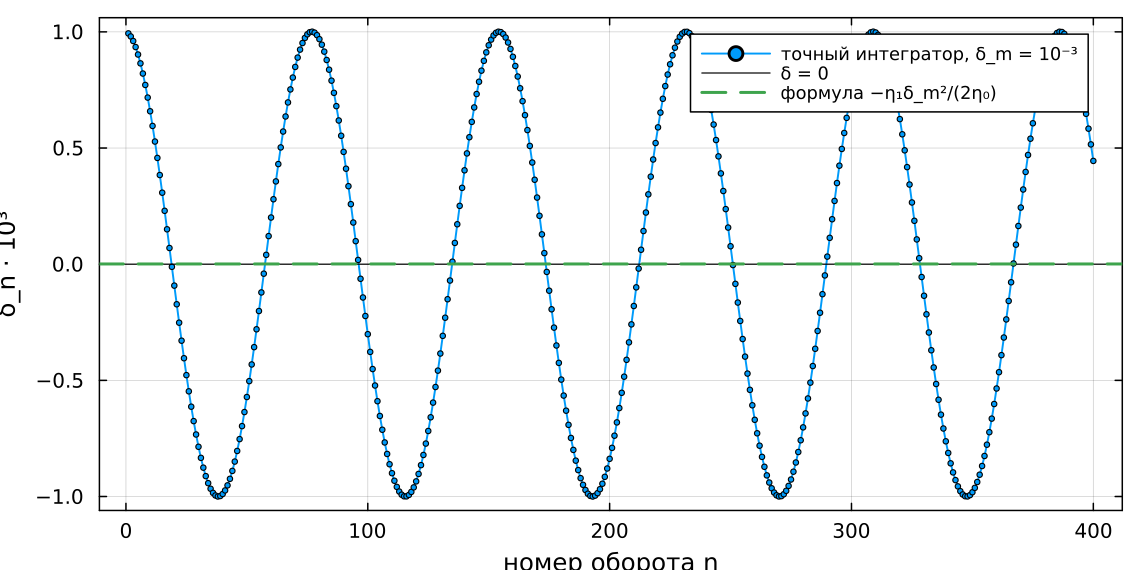
\includegraphics[width=0.92\textwidth]{figs/fig_01_delta.png}
\caption{Точный интегратор, $N=\vNshort$ оборотов. Размах $\vdHalf$. Горизонталь формулы $\vMoneSimple$ на этом масштабе совпадает с нулём.}
\end{figure}

\textbf{Вывод.} $\delta$ колеблется из-за ВЧ. Центр колебания глазом не виден: формула даёт $\vMoneSimple$, это в тысячу раз меньше размаха.
